\chapter{Epithelial Tissue and Vertex Dynamics}
\label{chap:intro}
\section{About Epithelial Tissue}
Epithelial tissue covers the interior and exterior surfaces of our bodies. Skin, the lining of the esophagus and intestines, the urethra, the lining of the lungs and the bronchioles are all made up of epithelial tissue. In this way, we can think of epithelial tissue as being the envelope in which our contents are packaged~\cite{ShapeFormation}; epithelial tissue is our interface with the outside world. 

\begin{figure}[hb]
\centering 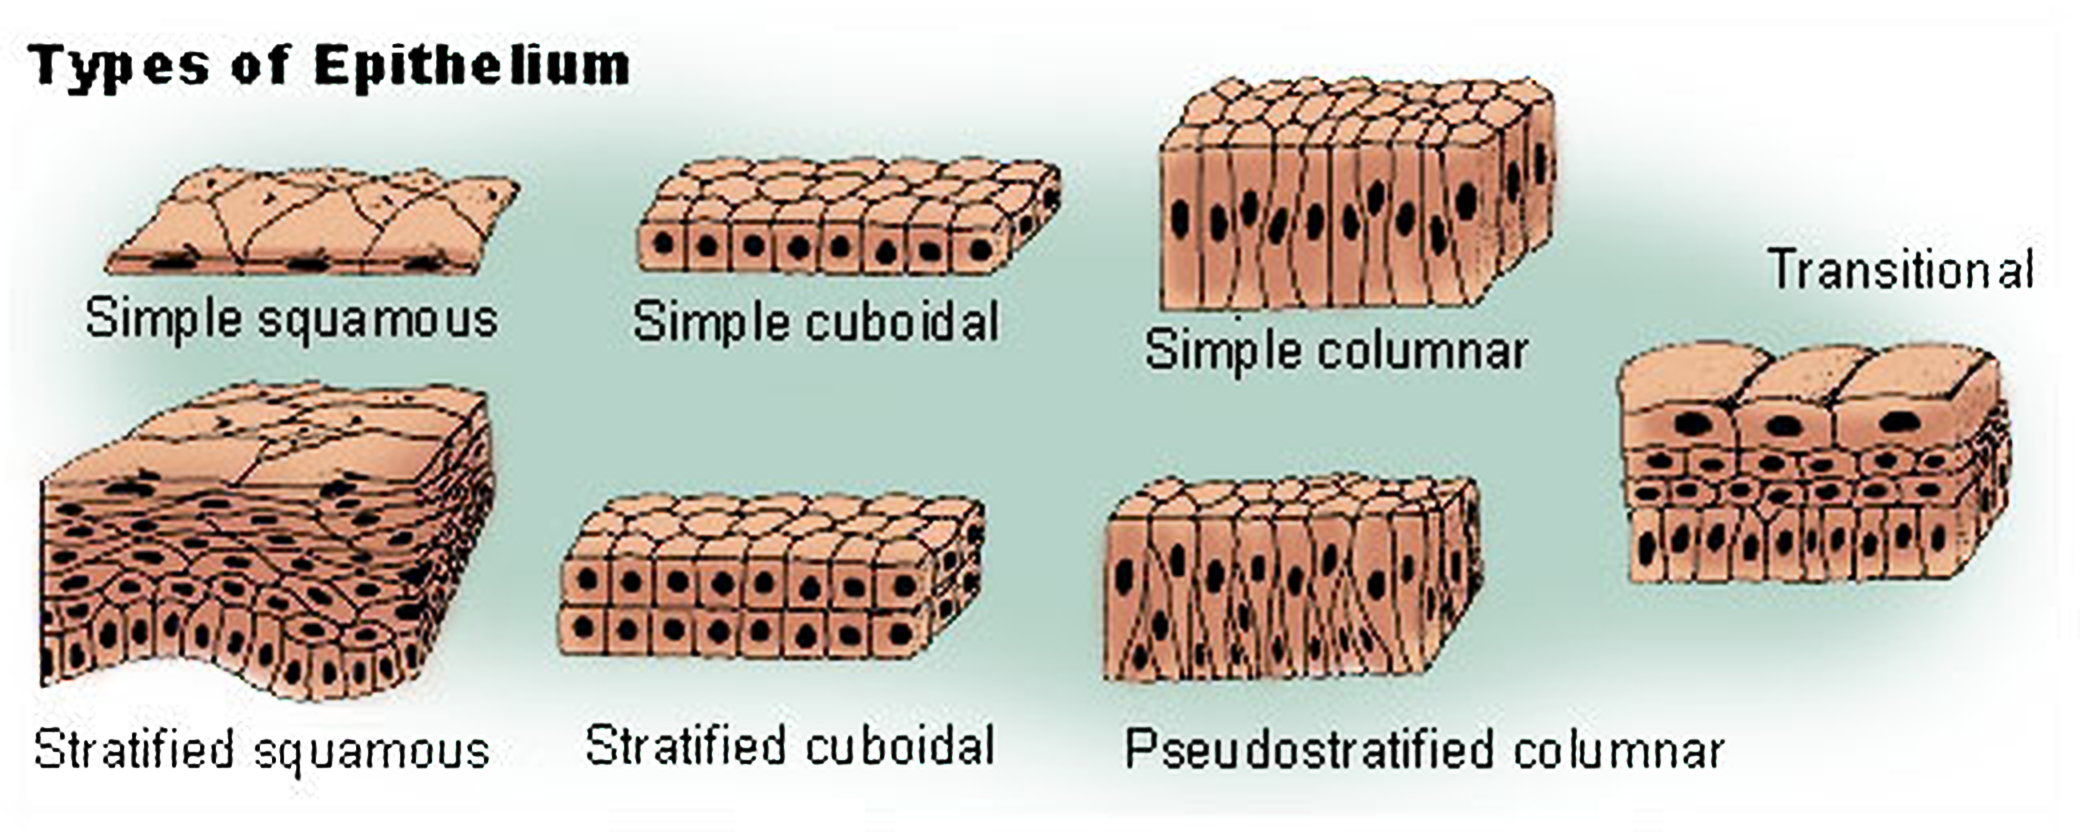
\includegraphics[width=\textwidth]{../diagrams/output.png}
\caption{The Types of Epithelial Tissue~\cite{Epithelium}.}
\label{fig:types}
\end{figure}

As Figure~\ref{fig:types} shows, there are many types of epithelial tissue in animals which vary in their number of layers and how the cells are shaped. Each of these types of cells are found in a different region of the body where they perform a specific function.  For example, the simple squamous epithelium is no more than one layer of cells thick, and the cells are much flatter than they are wide. Because these cells are well suited to allow diffussion across themselves, simple squamous tissue is found in the walls of blood vessels and in the alveoli in the lungs, where the diffusion of oxygen occurs. On the other hand, columnar cells are much taller than they are wide, and are thus well suited to absorption. These cells are found in the intestines where they absorb nutrients from passing food. Stratified squamous epithelia are several layers thick and line the esophagus and mouth and protect against abraision.

What all of these tissues have in common, however, is how amenable they are to computational modeling. The most easily modeled tissues are simple epithelia, which typically have near-uniform height, and very little difference in appearance between their apical and basal faces. This means that the cells can easily be approximated by a two dimensional mesh in which the surfaces where two cells touch are approximated by a line. Examples of 2D epithelial tissue simulations are presented in Figure~\ref{fig:fourgraphs}a,b. For an example of a 2D epithelial simulation on a three dimensional surface, see Figure~\ref{fig:fourgraphs}d. The 3D simulation of stratified tissue is more difficult to implement than a two dimensional model\footnote{Even a leading epithelial tissue simulator, Chaste~\cite{ChasteMain}, still does not have stable 3D modeling capabilities.}. For an example of one successful 3D model, see Figure~\ref{fig:fourgraphs}c.

\begin{figure}[ht]
    \centering
    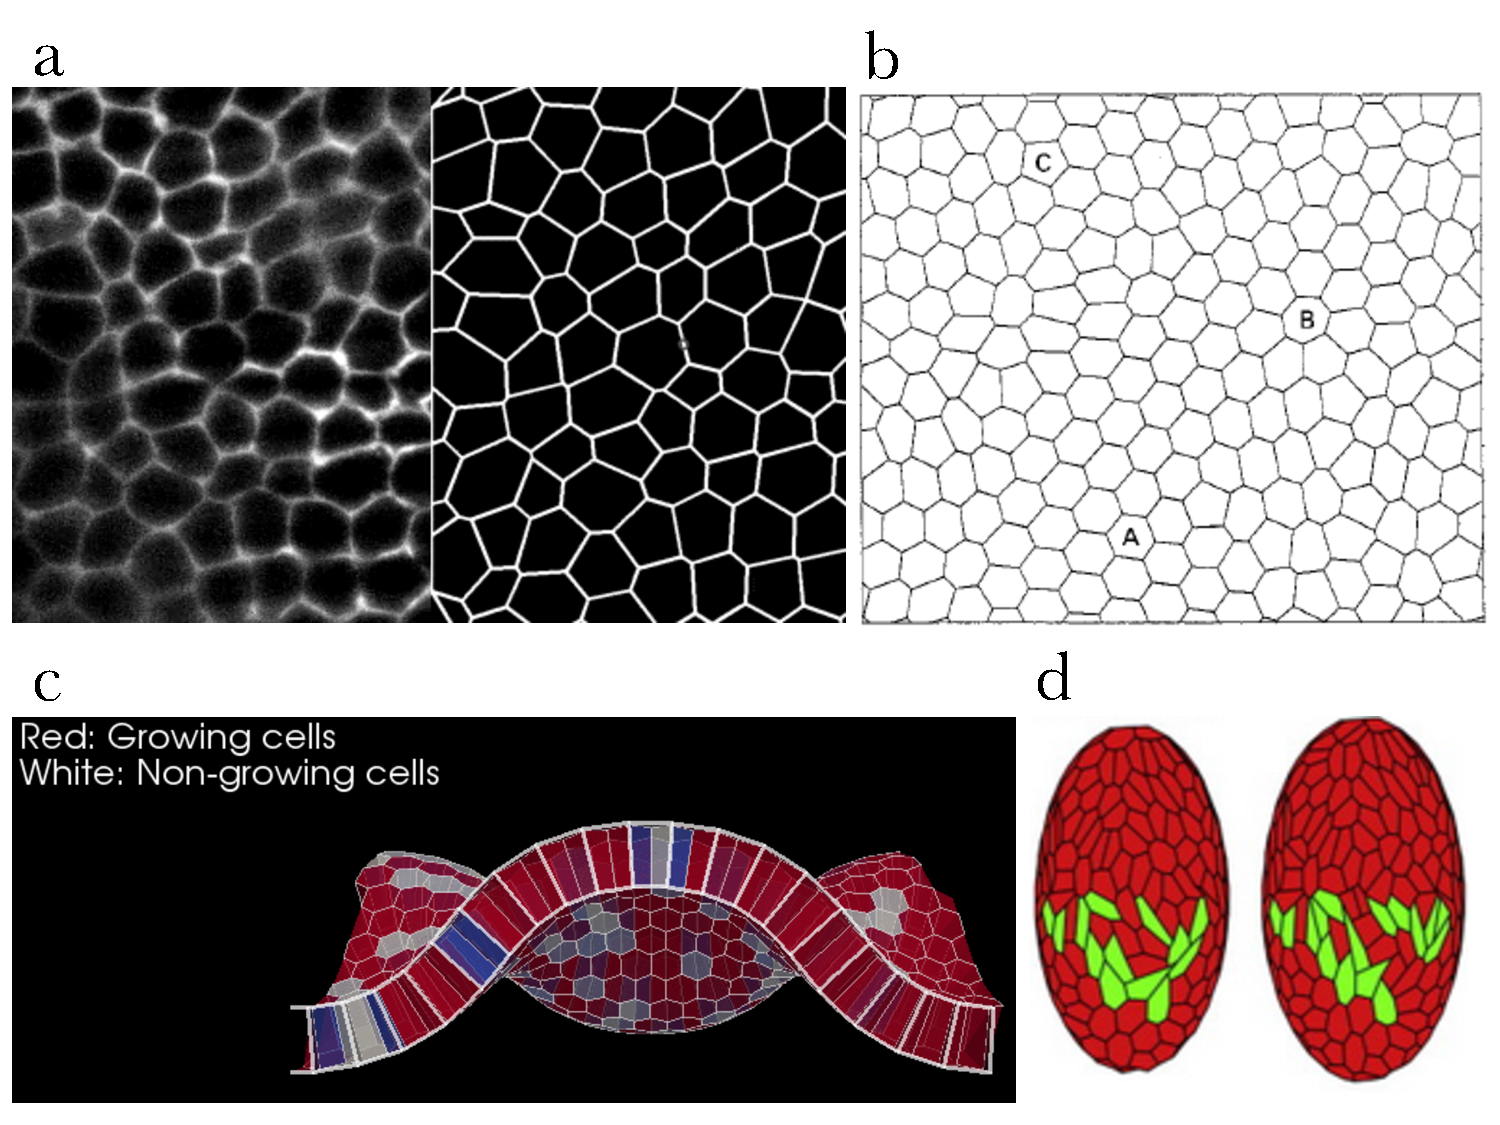
\includegraphics[width=\textwidth]{../diagrams/abcd3.pdf}
    \caption[Various Models of Epithelial Tissue]{Several screenshots illustrating the variety of epithelial tissue models. (a) A comparison of living tissue (left) to a simulation (right)~\cite{Yoshi}. (b) A diagram from the original Honda-Nagai paper~\cite{HondaNagai}. (c) A three-dimensional mesh of cells~\cite{Okuda1}. (d) A tissue developing on a surface~\cite{VertexModels}.}
    \label{fig:fourgraphs}
\end{figure}

Current modeling is producing great results in the field of epithelial tissue morphogenisis, equilibration, and wound healing. The Honda-Nagai model, which we will discuss in great detail below, successfully reproduced the wound healing of cats' corneas~\cite{WoundHealing}. This model has also been able to reproduce all of the essential dynamics of epithelial tissue~\cite{HondaNagai}.  Current imaging tools have enabled the recording of epithelial tissue dynamics \emph{in vivo}~\cite{Sokolow, Xiong}, providing a wealth of experimental data which can serve as either initial conditions for simulations, or as benchmarks to measure the accuracy of computational predictions. In turn, models of epithelial dynamics can provide insights into the physical parameters that govern tissue development, maintenance, and malady.

Other modeling communities share advanced, free, and parallel simulation codes. For example, consider LAMMPS~\cite{LAMMPS} for simulating atomistic materials, and CHARMM~\cite{CHARMM}, Amber~\cite{Amber}, and NAMD~\cite{NAMD} for the molecular dynamics simulation of biomolecules. Unfortunately, there are only a handful of codes in use for the simulation of epithelial tissue, and to the best of our knowledge only one of them is freely available~\cite{ChasteMain}. In this thesis I will present the basic ideas of \textbf{vertex dynamics models} of epithelial tissue, and then describe the implementation of one of them as a freely available modeling tool for the community.

\section{Modeling Epithelial Tissue} 
\label{sec:modeling}

A two dimensional \textbf{vertex dynamics model} of epithelial tissue is made up of vertices and edges~\cite{DirichletDomains}. The vertex dynamics model presupposes that the movement of cells in epithelial tissue can be approximated by the movement of edges and vertices. Some force is then proposed to guide epithelial cell movement according to an equation of motion that is solved via some numerical method.

Epithelial vertex dynamics has been a lively field of research since the 1970s because of several heartening results. Some researchers have had success modeling the morphogenesis of \emph{Drosophila} wing growth~\cite{Farhadifar}, whereas others have accurately reproduced the dynamics of corneal wound healing~\cite{WoundHealing}. In other research, simulations have faithfully captured the effects of laser perturbations to epithelial cell junctions~\cite{Yoshi}, and others have quantified parameters which are important in describing the formation of the epithelial envelope in \emph{Drosophila}~\cite{Sokolow}. Unfortunately, these results have not come from one standard model of epithelial tissue development, but from a variety of different, often irreconcilable, models. Two different approaches to epithelial simulation described below will clearly illustrate the variety of techniques in practice.

In the model developed by M. Weliky and G. Oster, forces due to osmotic pressure and contractile tension describe how vertices move~\cite{WO}. This model also allows for certain forces external to the tissue to be applied at each node. In the end, the force applied to each vertex in the mesh is given by
\begin{equation*}
F_i = F_{ext}+\sum\limits_{n=1}^N(T_{i-1}^n - T_{i+1}^n + P^n)
\end{equation*}
where $n$ is the index of the $n^{th}$ cell which touches vertex $i$. The force applied to vertex $i$ coming from cell $n$  is seen graphically in Figure~\ref{fig:WO}.
\begin{figure}[ht]
\centering
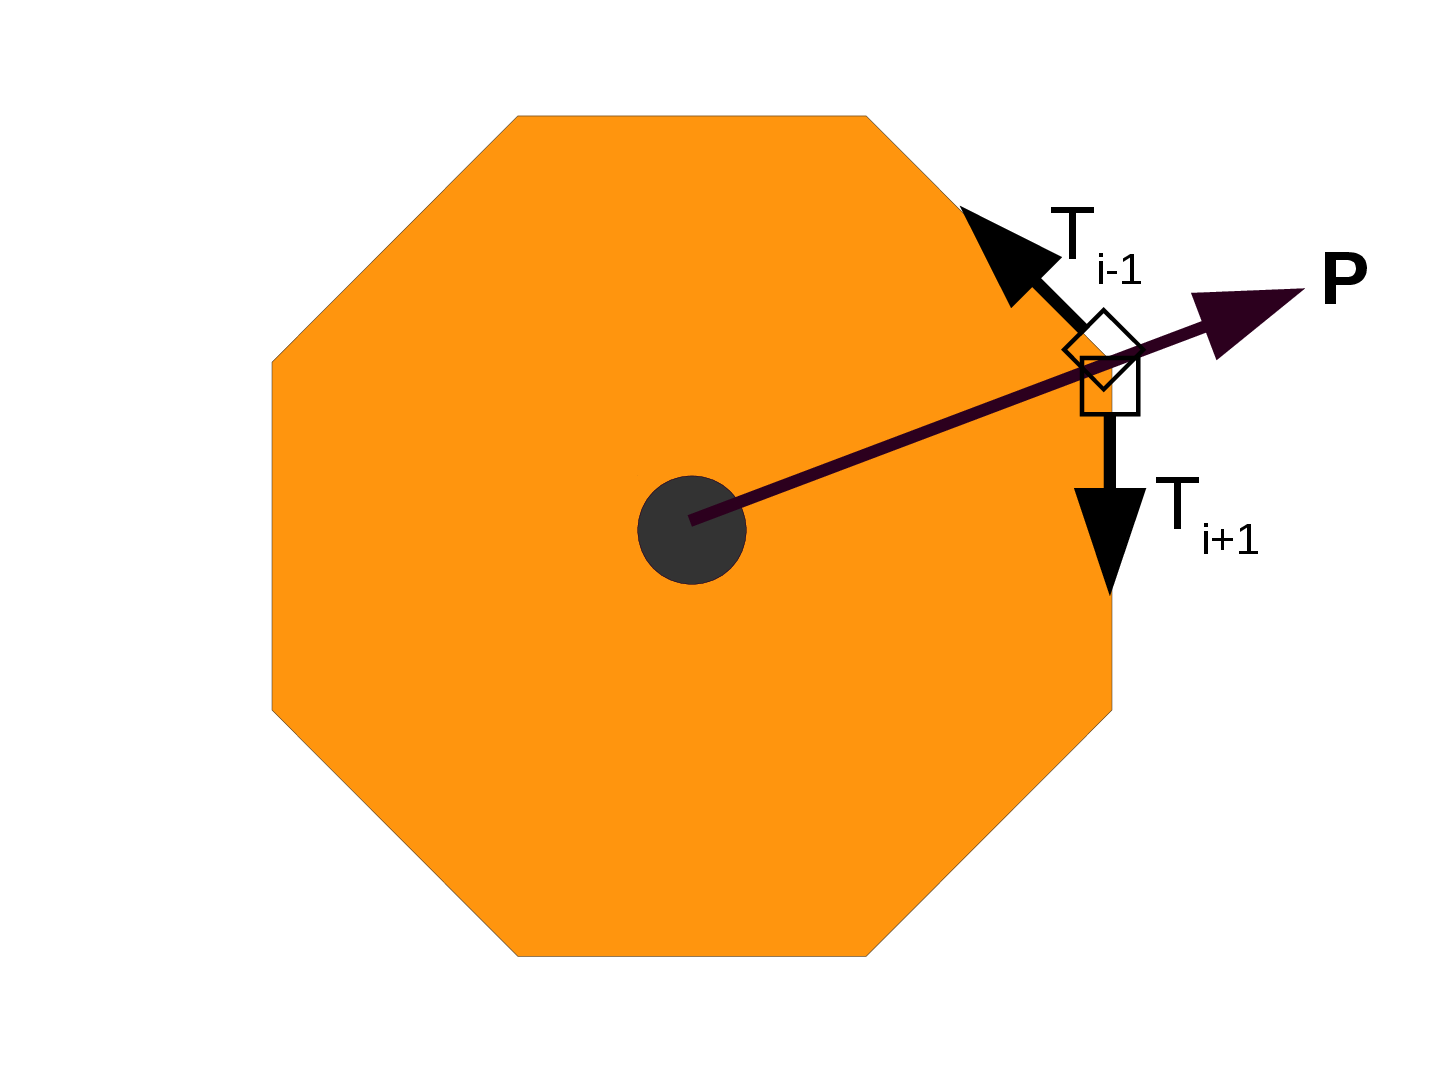
\includegraphics[width=0.5\textwidth]{../diagrams/welikyoster.png}
\caption{The Weliky-Oster Force.}
\label{fig:WO}
\end{figure}

In contrast, the model developed by H. Honda and T. Nagai takes an approach to modeling epithelial tissues rooted in the study of cellular structures~\footnote{Including living and non-living structures.}~\cite{VertDyn}.  In the fantastic review paper \emph{Soap, Cells, and Statistics}~\cite{Soap}, D. Weaire and N. Rivier argue for the existence of some natural mechanism underlying the development of epithelial tissue, columnar basalt formations, soap froths, grain growths, and other cellular structures, as they exhibit a great deal of similarity. For example, consider the images of epithelial tissue presented throughout this paper juxtaposed with the image of The Giant's Causeway in Northern Ireland in Figure~\ref{fig:cause}. The equilibrium states of these structures all contain primarily hexagonal cells, and three cells typically meet at any junction. There are some differences in the exact distribution of cell shapes, the presence of chemicals in biological tissues versus the absence of growth inducing chemicals in geological structures, and the active migration of biological cells versus the entirely passive movement of soap froths; still, the authors conjecture that the dominant principle behind all cellular dynamics is the seeking of a state with minimal potential energy.

\begin{figure}[ht]
\centering
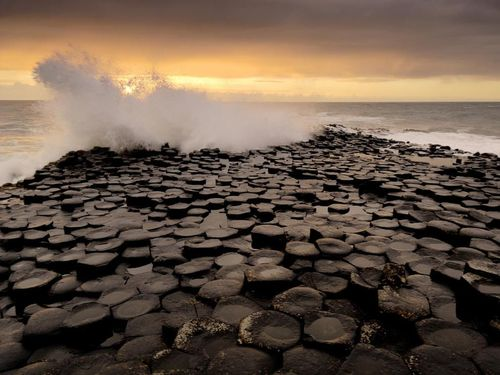
\includegraphics[width=0.5\textwidth]{../diagrams/resize_giant.jpg}
\caption{The Giant's Causeway. Adapted from~\cite{Giant}.}
\label{fig:cause}
\end{figure}

A very basic result from physics is the relationship between force and potential energy:

\begin{gather}
\vec{F} = (F_x, F_y, F_z)\\
W = -\Delta U(\vec{x}) = \int_{x_0}^xF_xdx+\int_{y_0}^yF_ydy+\int_{z_0}^zF_zdz\\
\nabla(-\Delta U(\vec{x})) = \nabla\Bigg(\int_{x_0}^xF_xdx+\int_{y_0}^yF_ydy+\int_{z_0}^zF_zdz\Bigg)\\
-\nabla U(\vec{x}) = \vec{F}
\end{gather}

In the Honda-Nagai model, the authors posit that dynamics of epithelial cell packing is dominated by their seeking a state with minimal potential energy. They describe several types of potential energy in a tissue, take a gradient of the energy function as described above, and then apply the resulting force to the vertices in the epithelial mesh~\cite{HondaNagai}.

While both the Honda-Nagai and the Weliky-Oster models successfully reproduce the topological and geometric properties of epithelial tissue, I have chosen to focus my efforts on the Nagai-Honda model. This was the original vertex dynamics model, it still enjoys considerable use by other researchers, and is of a form quite similar to that used by others~\cite{Farhadifar}.

\section{The Nagai-Honda Model}
\label{sec:force}
\subsection{How the Vertices Move}
In 1989, K. Kawaski showed that the dynamics of grain growth can be reduced to a first order system given by:
\begin{equation}
\label{eq:motion}
\eta\frac{dr_i}{dt} = F_i
\end{equation}
where $F_i$ denotes the force applied to vertex $i$, $r_i$ denotes the position of the $i^{th}$ vertex,  and the left hand side is the velocity of the vertex multiplied by a positive drag coefficient, $\eta$~\cite{1989Kawasaki}. This is equivalent to $m_i\frac{d^2r_i}{dt^2} + \eta\frac{dr_i}{dt} = F_i$, in which the 
inertial term is considered to be much smaller than the drag term.

Based upon the notion that biological cells move in a way quite similar to high temperature crystallites\footnote{Often referred to as grain growth.}, the Honda-Nagai model has equation~\ref{eq:motion} as its basis. The force on the right hand side of the equation is in turn defined as the gradient of an energy function, since the model presupposes that the tendency towards a state of lower potential energy is the guiding principle behind epithelial tissue equilibria. The energy function is composed of three terms which reflect the properties of biological cells.

The first two potential energy terms come from the assumption that the cell is elastic, and that the cell wants to return to a target shape. Therefore, the first two energy terms are of the harmonic form: 
\begin{equation}
C(x-x_0)^2
\end{equation}
where $x$ is some physical quantity, and $C$ is some constant. The plot of this energy is therefore a parabola with a minimum at $x =  x_0$, and the farther the quantity $x$ strays from the equilibrium, the steeper its gradient will be, and the more forcefully it will want to return to equilibrium.

The third energy term is an adhesion energy, which is proportional to the amount of interfacial surface area between a cell and its neighbor. There is a successful theory in biology called the \textbf{differential adhesion hypothesis} which attempts to account for certain cellular distribution phenomena through adhesive binding tendencies. The theory essentially says that certain cells tend to bond more tightly to cells of type A than to cells of type B due to the presence or absence of different adhesion proteins in the membranes of these cells~\cite{DA}. In proliferating tissues, this difference in binding energies leads to cell segregation and the formation of structured tissues and organs. 

The precise definitions of the potential energies are:

\begin{enumerate}
\item The deformation energy term $U_D$ is given by \\ 
\begin{equation}
U_D = \lambda(A - A_0)^2
\end{equation}
 where $A$ is the cell area, $A_0$ is the target cell area, and $\lambda$ is some positive constant.
\item The membrane surface energy term $U_S$ is given by
\begin{equation}
U_S = \beta(P - P_0)^2
\end{equation}
 where $P$ is the cell perimiter, $P_0$ is a target perimeter, and $\beta$ is some positive constant.
\item The cell-cell adhesion energy $U_A$ is given by
\begin{equation}U_A = \displaystyle\sum\limits_{j = 1}^{n}\gamma_{j}d_{j}\end{equation}
where $n$ is the number of vertices in the cell, $\gamma$ is some constant for the boundary in question between one cell and another, and $d$ is the distance between one vertex and the next in a counter clockwise fashion. Note that in two dimensions the boundary is a distance $d$, but in three dimensions it would have to be the area of a cell face. 
\end{enumerate}

In total, the potential energy in a sheet of $N$ cells is given as:
\begin{equation*}
U = \sum\limits_{c = 1}^N\left(\lambda_c(A_c - A_{0_c})^2 + \beta_c(P_c - P_{0_c})^2 + \sum_{edges\in c}\gamma_{edge}d_{edge}\right)
\end{equation*}

 As seen in~\cite{ChasteMain}, the negative gradient of this potential energy with respect to vertex $i$ is:

\begin{equation}
\label{eq:force}
\begin{split}
F_i = -\displaystyle\sum_{l\in N_i}(2\lambda(A_l - A_{0_l})\nabla_iA_l + 2\beta(C_l - C_{0_l})(\nabla_i d_{l, I_l-1}+\nabla_i d_{l, I_l}) +\\ \gamma_{l, I_l-1}\nabla_i d_{l, I_l-1} + \gamma_{l, I_l}\nabla_i d_{l, I_l}
\end{split}
\end{equation} 
where $l$ is the $l^{th}$ cell containing vertex $i$, given a counter clockwise orientation. $I_l$ is the local index of node $i$ in element $l$. A detailed derivation of the force follows, as in~\cite{ChasteMain}.

 The area of a convex cell made up of $n$ vertices is given by Gauss's shoelace formula:
\begin{equation}
A = \frac12\sum\limits_{i=1}^n\Big(x_iy_{(i+1)mod(n)}-x_{(i+1)mod(n)}y_i\Big)
\end{equation}
Therefore, the gradient with respect to vertex $i$ is given by:
\begin{equation}
\nabla_i A_l = \frac12
\Big(
y_{I_l+1} - y_{I_l-1},\;\;x_{I_l-1} - x_{I_l+1}
\Big)
\end{equation}
 where the subscripts $l$ denote that $x$, $y$ are in cell $l$. The subscripts are local indices in the cell $l$, and the orientation of vertices is counterclockwise. The circumference is given by:

\begin{equation}
P = \sum\limits_{j=1}^Nd_j = \sum\limits_{j=1}^N\sqrt{(x_{j+1} - x_j)^2 + (y_{j+1} - y_j)^2}
\end{equation}
Therefore
\begin{gather}
\nabla_iP = \nabla_id_{i-1} + \nabla_id_i
\end{gather}
and
\begin{equation}
\nabla_id_{l, j} = \frac1{d_{l, j}}
\Big(
x_{j+1}- x_j,\;\; y_{j+1} - y_j
\Big)
\end{equation}
Substituting the above values into the equation:
\begin{equation}
-\nabla_iU = -\nabla_i(U_D + U_S + U_A) = F_i
\end{equation}
gives the force described in equation(~\ref{eq:force}).

\subsection{Topological Changes to the Mesh}
\begin{figure}
    \centering
    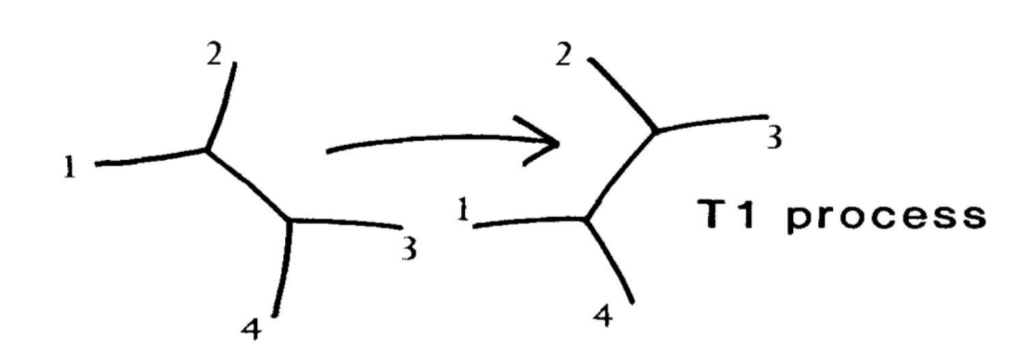
\includegraphics[width=\textwidth, keepaspectratio]{../diagrams/t1.png}
    \caption{A T1 Swap.}
    \label{fig:t1}
\end{figure}
There is emprirical evidence that nearly all vertices in a sheet of epithelial tissue have coordination number three (most vertices have three incident edges)~\cite{EpithelialTopology}. This observation has led many researchers in the field of cellular structures to consider what sort of topological changes can occur in meshes of cells without changing their connectivity~\cite{Soap}.  As it turns out there are three possible changes called the T1, T2 and T3 swaps, and the original Honda-Nagai Model implements the first two.

 The T1 swap, illustrated in Figure~\ref{fig:t1}, is also called a ``neighbor exchanging swap" because two cells that were adjacent cease to be neighbors and two cells that were not adjacent become neighbors. The T1 swap occurs when two vertices become critically close to each other, and instead of allowing the vertices to collide we rotate the offending edge. There is no specification in the literature about how to rotate the edge, but the natural choice is to turn the edge by 90 degrees. In nature this should correspond to two vertices getting very close, colliding, and then flattening out into an edge. The Honda-Nagai model performs this action discretely as a simplifying measure to avoid having to handle the momentary degree four vertex.


\begin{figure}
\centering
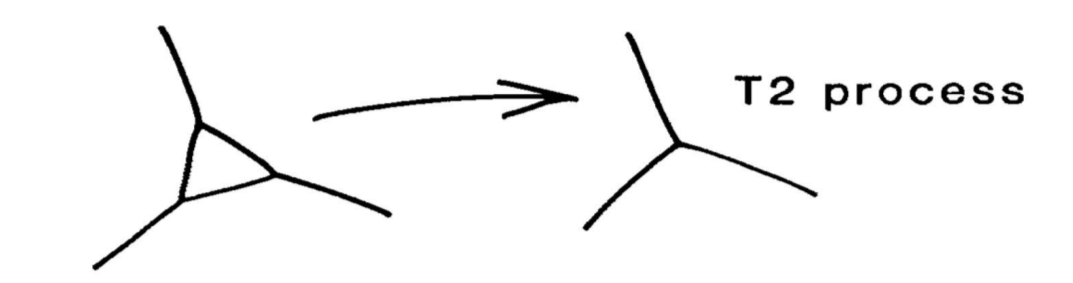
\includegraphics[width=0.8\textwidth, keepaspectratio]{../diagrams/t2.png}
\caption[A T2 Swap]{A T2 Swap.}
\label{fig:t2}
\end{figure}

The second topological change is the T2 swap, which is also known as ``cell removal''. A T2 swap occurs when an edge of a triangular cell becomes too small and the cell is deleted and replaced by a single vertex located at the centroid of the cell (Figure~\ref{fig:t2}).

\subsection{Selection of Parameters}
The basic vertex dynamics model requires the user to specify the $A_0$, $P_0$, and $\gamma_{edge}$ parameters for each cell, as well as a value for the drag coefficient $\eta$ and the integration timestep $dt$. The equations in this model are dimensionless. I will not undertake a discussion of how to derive the dimensionless model from the dimensional model, but for the curious reader this is all laid out in~\cite{HondaNagai}. Typically, one would not choose the values of the aforementioned parameters, but would instead have some dimensional biological data and go through the necessary conversion steps to use them in the simulation~\cite{NewOkuda}.

Interestingly, I haved found very few explicit statements of the parameters used in simulation (exceptions are~\cite{WoundHealing, ChasteMain, NewOkuda}). As Honda has said, ``We do not have accurate values for the cell parameters at present''~\cite{Honda3D}.  Very recently, new imaging techniques have permitted the \emph{in vivo} observation of epithelial tissue morphogenesis~\footnote{Morphogenesis is the development of shape in an organ or organism.}~\cite{Sokolow, Xiong} and this will likely open new doors for a more accurate parameterization of current models, or perhaps even for the reformulation of the expressions for forces and potential energies. 

\begin{figure}[ht]
\centering
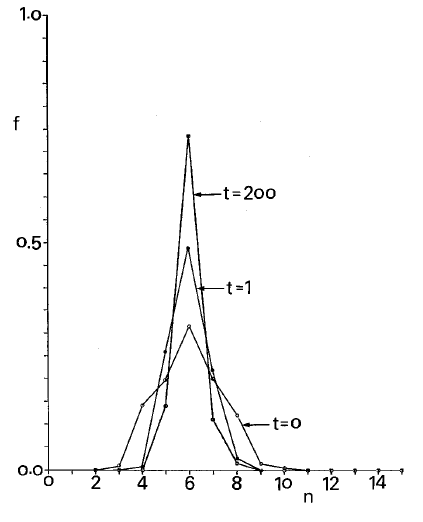
\includegraphics[width=0.5\textwidth]{../diagrams/distibutionHonda.png}
\caption[Distribution of Cell Shapes]{The distribution of cell shapes as a function of time in the original Honda-Nagai Model. Adapted from~\cite{HondaNagai}}
\label{fig:hnm}
\end{figure}

In the case of the Honda-Nagai Model, however, there is little difference between equilibrium states attributed to various parameter choices (See Chapter~\ref{chap:Epithelium}). One of the parameter-independent defining characteristics of the Honda-Nagai model is the strong tendency toward six-sided cells in equilibrium (Figure~\ref{fig:hnm}).  Yet, it has been shown that different parameter values coupled with other mesh changing operations (such as oriented cell division) can cause drastically different types of morphogenesis~\cite{Overview}. For example, drosophila wings, with their highly oriented divisions, have been shown to contain approximately 80\% hexagonal cells whereas simulations of tissues with purely stochastic divisions converge to  approximately 47\% hexagons~\cite{EpithelialTopology}. While all epithelial tissue has a strong tendency towards achieving an equilibrium dominated by hexagons, the width of the distribution of cell shapes differs by cellular structure and, hence, by parameter choices~\cite{Soap}. 


\section{Further Remarks About Epithelial Tissue Modeling}
Over the years, various modifications and improvements have been made to the Honda-Nagai model. These changes involve new ways of specifying the potential energy, adding new cell dynamics, and changing the connectivity of the mesh. In this section I will discuss some of these advances, as well as present some important mathematical theory underlying epithelial tissue models.


\begin{figure}
\centering
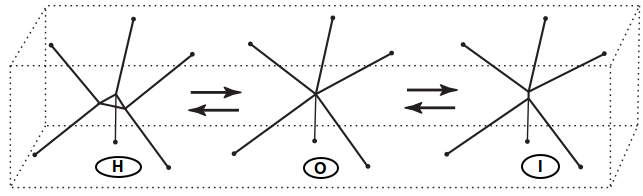
\includegraphics[width=\textwidth]{../diagrams/hoi.png}
\caption[The HOI swap.]{The HOI swap. \emph{H} configutation(left), \emph{O} configuration (center), \emph{I} configuration (right). Adapted from~\cite{Honda3D}.}
\label{fig:hoi}
\end{figure}

\subsection{Three dimensional models: Honda-Nagai and Okuda.}
Honda and Nagai also implemented their model in three dimensions and used the same equation of motion for the tissue~\cite{Honda3D}. However, while the vertices in two dimensions all meet at the junction of three edges,  in three dimensions the vertices meet where four edges are coincident, and each edge is touched by four polygonal faces. A new type of topological change handles the new connectivity, as the T1 and T2 swaps work only on two-dimensional meshes. The so-called HOI swap (Figure~\ref{fig:hoi}) looks at all of the edges in the mesh and finds the edges measuring less than $\delta$; then, it proceeds on a case by case basis. If the edge lies on a triangle, then it is of the \emph{H} form, and the swap goes from left to right (as indicated in Figure~\ref{fig:hoi}). Otherwise, the edge is of the \emph{I} form, and the transformation goes from right to left~\cite{Honda3D}. The Honda-Nagai model in three dimensions has been successful in describing how embryonic epithelial cells grow in a plane at the expense of not proliferating in the orthogonal direction, but is not the only 3D epithelial growth model.

\begin{wrapfigure}{r}{0.5\textwidth}
  \begin{center}
    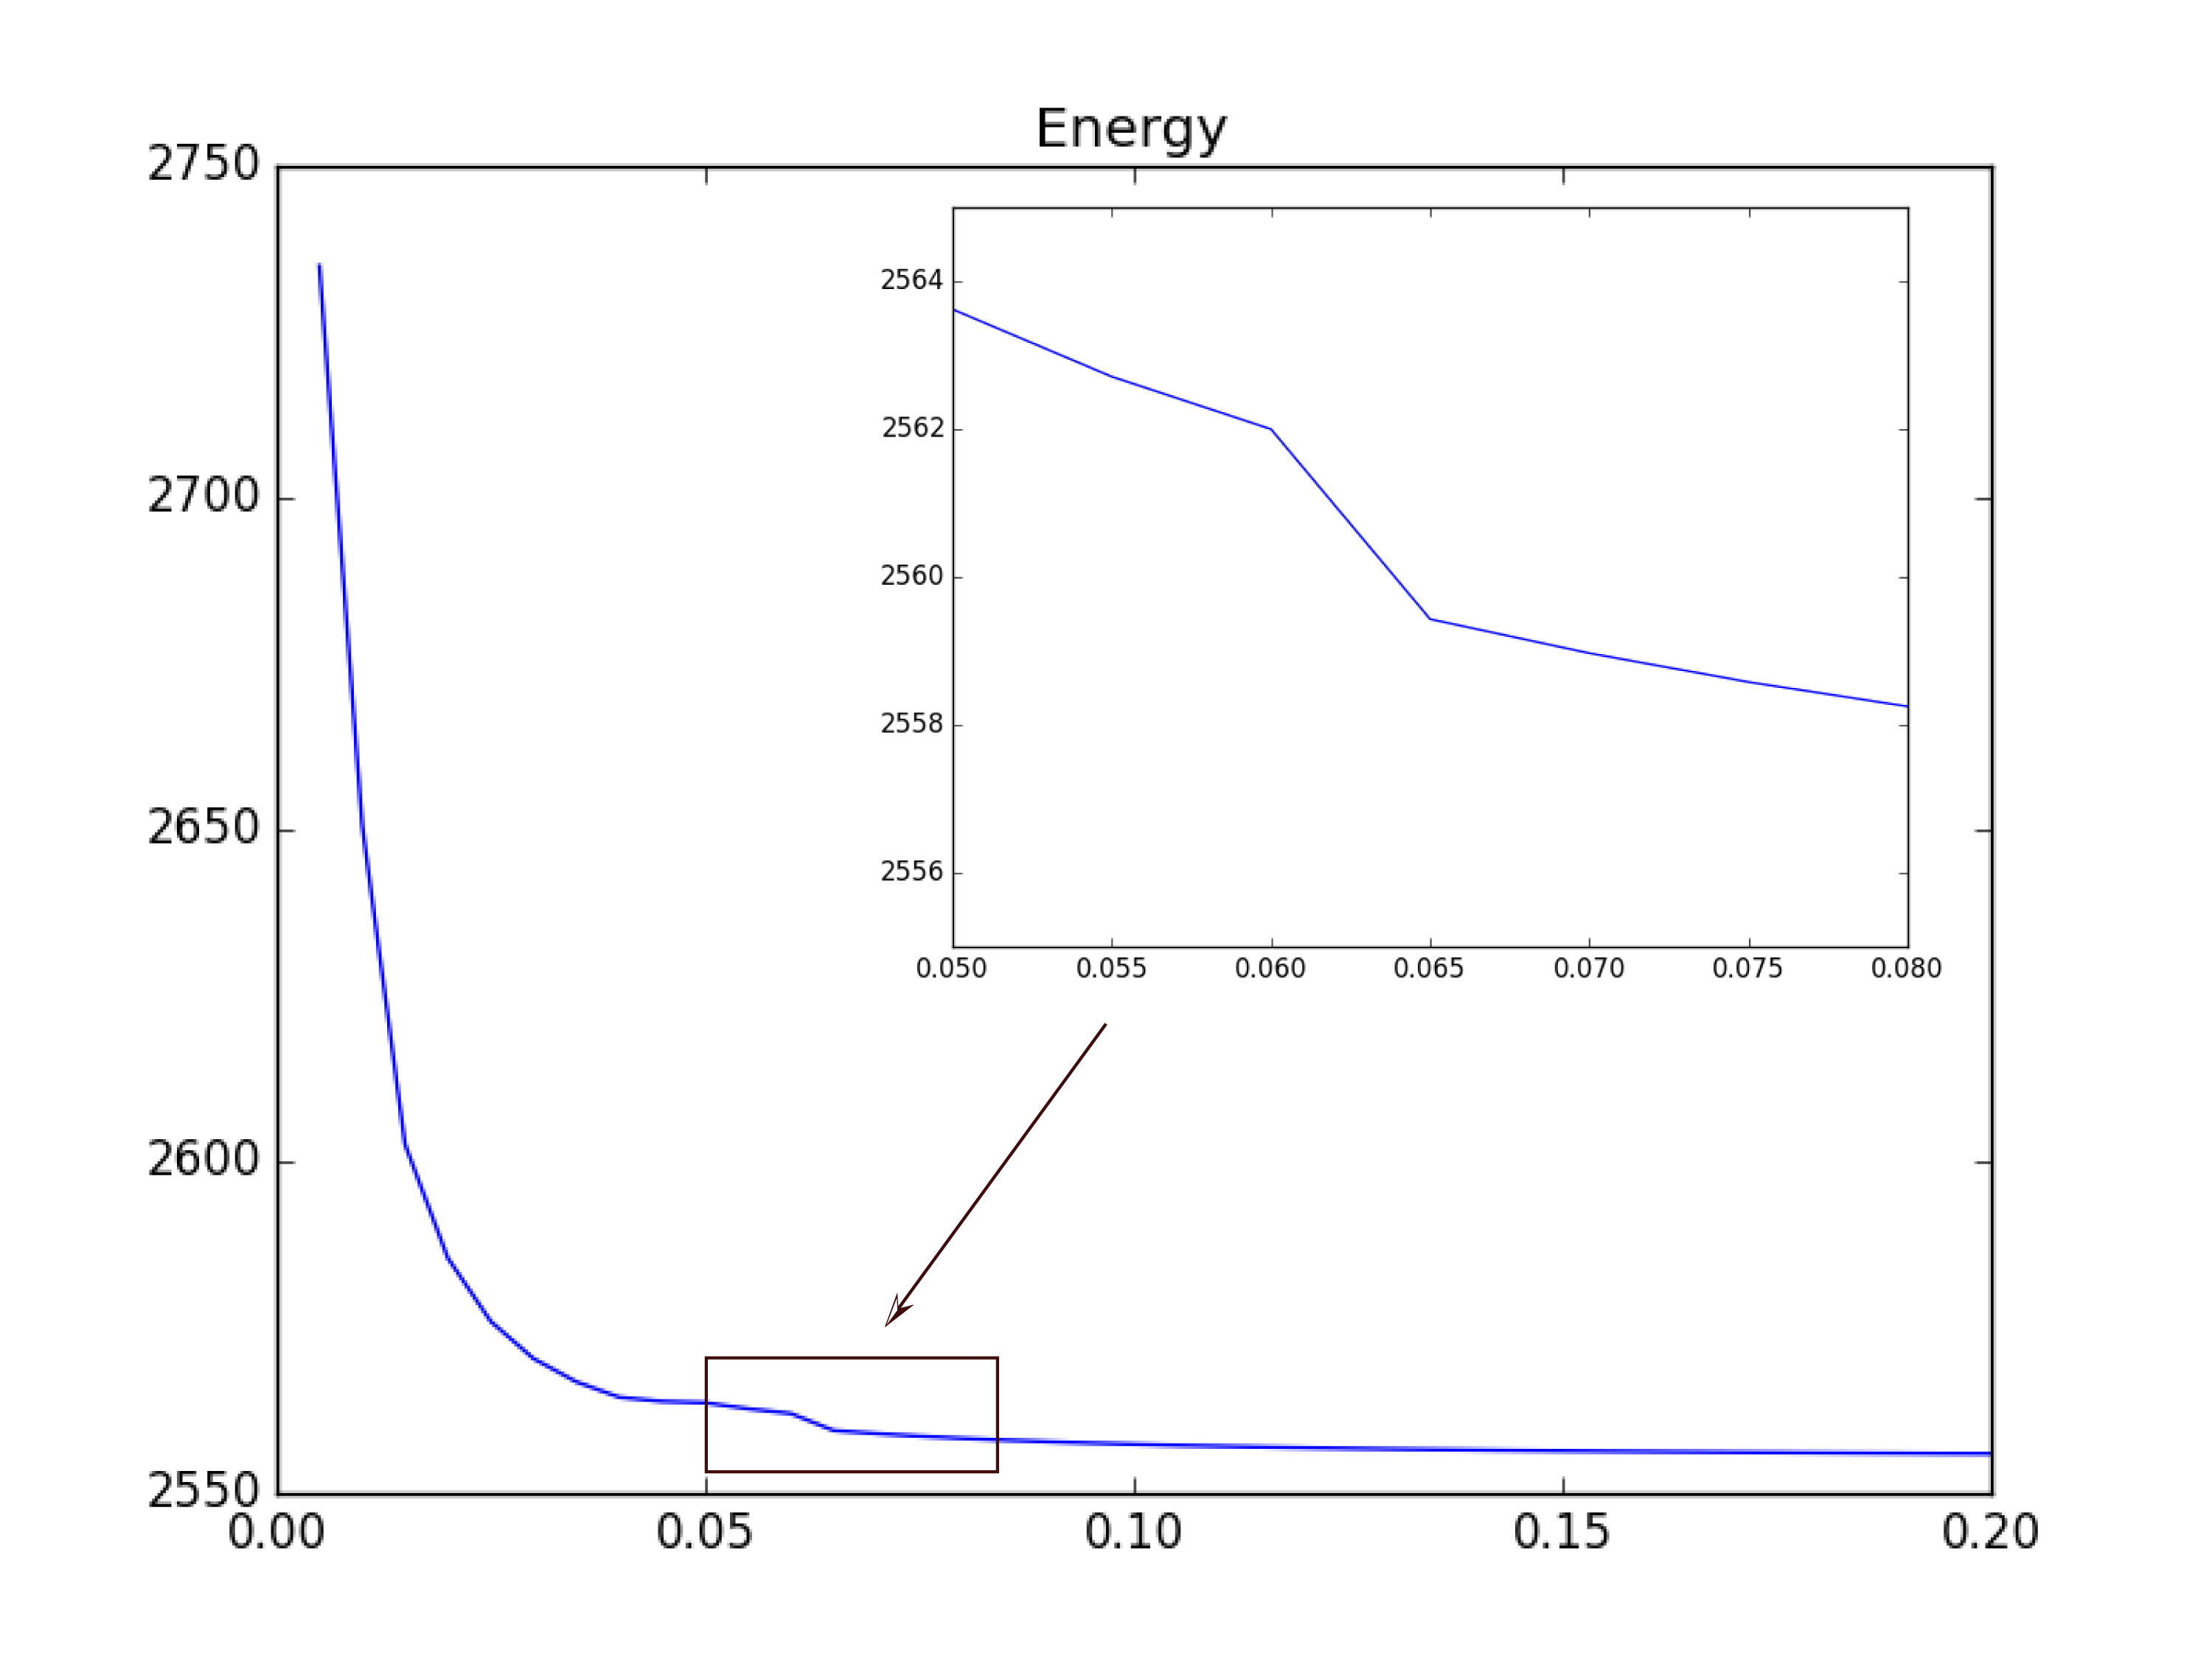
\includegraphics[width=0.48\textwidth]{../diagrams/jump.png}
  \end{center}
\caption[A non-smooth energy curve.]{A jump in the potential energy. The reconnection scheme of the Honda-Nagai model can 
result in curves which are not smooth under certain circumstances.}
\label{fig:jump}
\end{wrapfigure}

The 3D vertex dynamics models recently developed by Okuda and co-workers take a slightly different approach than Honda and Nagai. The new models of epithelial tissue morphogenesis feature an altered cell reconnection model (Reversible Network Reconnection, or, RNR) which allows new tissue dynamics to develop~\cite{Okuda1}, and include a new viscosity term in the equation of motion which gives the model more physical plausibility~\cite{Okuda3}.

The proposed reconnection scheme contrasts with the Honda-Nagai model in that there are no large inconsistencies in the energy output (Figure~\ref{fig:jump} and Figure~\ref{fig:g1}). The principal idea behind the RNR is that a triangular element ought not be reduced to a point unless \emph{all} of its edges are critically small, whereas in the two-dimensional Honda-Nagai model a T2 swap (and in the three-dimensional model, an HIO swap) occurs when only one edge of a triangular face is smaller than $\delta$. This can lead to jumps in potential energy, as well as generate artifical tissue dynamics which only occur because edges which are larger than the approximated zero length ($\delta$) are forced to zero. Due to the fact that a triangle is forced to a vertex, the occurence of an oscillation through several T2/HOI swaps at a vertex is not seen by the model. The two drawbacks to the RNR model are that it may not produce quality results when simulating tissues in which topological irreversibility is a defining feature~\cite{CellSurf}, and that the model can sometimes produce topologies which are not computable by the software implementing it, i.e. when one edge of a triangle becomes critically small, while the other two remain long, and the triangle becomes a double edge between two vertices~\cite{Okuda3}).

Okuda's other innovation was the introduction of a new viscosity term into the equation of motion for a vertex, giving:
\begin{equation}
F_i = \eta_i(\frac{dr_i}{dt} - \vec{v_i})
\end{equation}
where the $\vec{v_i}$ is a vector which describes the viscous force acting on a vertex as a result of its local interactions with neighboring vertices. Observations of growing tissues show that the viscosity of a growing tissue is inhomogeneous and depends upon the cells types in a region as well as the membranes interacting with the cells, yet prior vertex models did not take this into account. For this reason, the Honda-Nagai 3D model was unable to capture the morphogenetic dynamics seen in~\cite{Mao}, while the Okuda model was.


\subsection{Similar Models of Potential Energy}
Interestingly, as mentioned in section~\ref{sec:modeling}, the Honda-Nagai form for the energy in a vertex is quite similar to the form developed by Farhadifar~\cite{Farhadifar}. The Farhadifar formulation is:
\begin{equation}
E_i = \sum\limits_{cells}\frac K2(A - A_0)^2 + \sum\limits_{edge}\gamma_{edge}d_{edge} + \sum\limits_{\alpha}\frac\beta2P_\alpha^2
\end{equation}

Remember the formulation of the Honda-Nagai energy:
\begin{equation*}
U = \sum\limits_{cells}\left(\lambda(A_c - A_{0_c})^2 + \beta(P_c - P_{0_c})^2 + \sum_{edges_c}\gamma_{edge}d_{edge}\right)
\end{equation*}

The equations are nearly identical, except that the Farhadifar model asserts that the cell perimeter persistently tries to collapse the cell ($P_0=0$), while the potential energy due internal pressure ($A_0\ne0$) resists this tendency. Nevertheless, the topological results of this model are not wildly different from the Honda-Nagai results~\cite{Farhadifar}.

\subsection{The T3 Swap}
The T3 swap is also known as ``mitosis'' or ``cell division''. Cell division was not a part of the original Honda-Nagai Model~\cite{HondaNagai} that dealt with the equilibration of a fixed number of cells. However, during proliferation cells divide, and computational models need to take into account tissues with varying numbers of cells. The challenge with implementing the T3 swap is that there are infinitely (within the bounds of floating point arithmetic) many choices about where to divide a cell, and there are several competing opinions (though no unanimouslly accepted theory) about how the division is oriented. Some cells divide along their longer axis, which is known as the `Hertwig's Long Axis Rule', but global tissue stress and local cell geometry are also thought to affect the orientation of mitosis~\cite{Order, Orientation}. The computational realization of a T3 swap is trivial, as the swap occurs by placing two new vertices along the edges of a cell and joining them by a new edge. The trouble is that there is no specification about which edges ought to have vertices implanted, or where to insert these vertices. The choice of where to divide a cell in a proliferating tissue can have profound effects upon the geometric appearance of a tissue - indeed, improperly oriented cell divisions are an indicator of cancer~\cite{EpithelialTopology, misaligned}. 
\begin{figure}
\centering
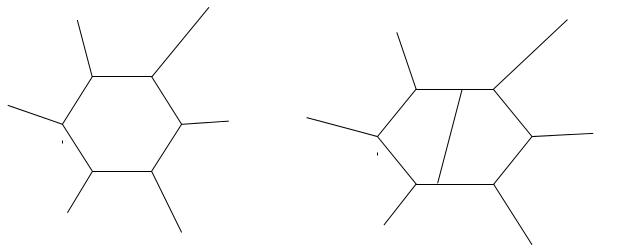
\includegraphics[width=\textwidth]{../diagrams/t3.png}
\caption[The T3 Swap.]{The T3 Swap.}
\label{fig:t3}
\end{figure}

\subsection{The Euler Characteristic and Its Implications}
The majority of current vertex dynamics models assume that all vertices have a coordination number of 3, since empirical evidence shows that the vast majority of cells have this property~\cite{EpithelialTopology,Overview}. In this section I will expand upon some observations made in~\cite{Soap} that deal with this phenomenon. \textbf{Euler's Formula} is an equation which relates the number of edges, faces, and vertices in a graph or polyhedron. An invariant $\chi$ relates the faces, edges, and vertices as follows:

\begin{equation}
\chi = V - F + E
\end{equation}

The invariant depends upon the graph or polyhedron in question. We will ignore the exact value of $\chi$ and simply use the fact that it is a constant. We know that each vertex connects to exactly three other vertices. Then we notice that all edges have two vertices, and that all vertices are connected to three edges. Inititally, our intuition tells us that there should be three times as many edges as vertices, which leads us to the incorrect formula:
\begin{equation}
3V = E
\end{equation}
But then we notice that if we consider all of the vertices in the mesh, we count each edge twice, so we divide by two and then simplify to get:
\begin{equation}
3V = 2E
\end{equation}

Similarly, if we consider how to relate the number of edges to the faces in the mesh, we conjecture that the number of edges in the mesh is equal to the sum of the products of cell shapes by the sides, $k$,  per shape. More clearly, we might guess the following:
\begin{equation}
\sum_{k=3}^N kF_k = E
\end{equation}
where $N$ is the highest number of edges in any cell in the mesh. But in this way we have again counted all of the edges twice, so the true number of edges must be the summation above divided by 2. We simplify the equation to get
\begin{equation}
\sum_{k=3}^N kF_k = 2E
\end{equation}
Now, we are able to reduce Euler's Formula to one variable using the relationships given above.
\begin{gather}
V - F + E = \chi\\
\frac{2E}3 - F + E = \chi\\
\frac{5E}3 - F = \chi\\
\frac{\sum_{k=3}^N kF_k}{6} - F = \chi\\
(\frac{\sum_{k=3}^N kF_k}{F} - 6)F = 6\chi
\end{gather}

Biological cells are very small, and an epithelial tissue is composed of many cells, so we assume that $F\to\infty$ and then immediately notice that the expression in parentheses must tend to zero as $F$ goes to infinity, or else the left hand side of the above equation will not approach the constant $6\chi$. From here it is easy to see that the introduction of a finite number of vertices with coordination number higher than three will not affect this result in the limiting case. Of course we have no reason at this point to assume that there is even one cell in the mesh with exactly six edges. It is feasible that the tissue is entirely be made up of five and seven sided cells. Nevertheless, empirical evidence shows a strong central tendency in the distribution of cell shapes. Whenever a cell tries to stray from the average, there are computational means (such as the T3 swap) of recentering the distribution at 6 sides.

The choice to impose degree three on each vertex is not one hundred percent consistent with nature, but has been a part of most models of epithelial tissue.  It is a simplifying assumption that \emph{rosettes} (epithelial cells organized radially about one vertex which has degree greater than or equal to 4) do not change the global dynamics of the development of an epithelial tissue.  Recent computer vision developments~\cite{rose} have made it easier to detect rosettes in epithelial tissue samples and may in the future provide information about the number of these formations, or evidence that rosettes are an important feature of epithelial tissue. Models would need to be revised to handle the introduction of vertices of higher degree.

